\begin{pa} \label{PA:0.5}
A tall water tower is swaying back and forth in the wind.  Using an ultrasonic ranging
device, we measure the distance from our device to the tower (in centimeters) every two
seconds with these measurements recorded below.  

\medskip

\begin{tabular}{| c | c | c | c | c | c | c | c | c | c | c | c |}
\hline
Time (sec) & 0 & 2 & 4 & 6 & 8 & 10 & 12 & 14 & 16 & 18 & 20 \\
\hline
Distance (cm) & 30.9 & 23.1 & 14.7 & 12.3 & 17.7 & 26.7 & 32.3 & 30.1 & 21.8 & 13.9 & 12.6 \\
\hline
\end{tabular}

% \begin{enumerate}
\ba
\item Use the coordinate plane below to create a graph of these data points.
    \begin{center}
%         \begin{tikzpicture}
%             \begin{axis}[axis lines=center, xmin=-0.5, xmax=20, ymin=0, ymax=40,
%                 xtick={2,4,6,8,10,12,14,16,18,20}, ytick={5,10,15,20,25,30,35,40}, grid,
%             xlabel={Time (sec)}, ylabel={Distance (cm)}]
%                 \addplot[smooth] {0*x};
%             \end{axis}
%         \end{tikzpicture}
        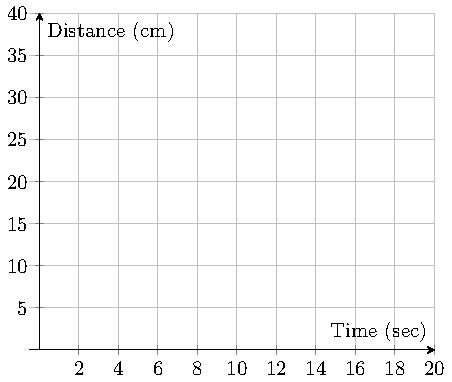
\includegraphics[width=0.5\columnwidth]{figures/0-5-fig1.pdf}
    \end{center}
\item What is the water tower's maximum distance away from the device? % 32.3 cm
\item What is the smallest distance measured from the tower to the device? % 12.3 cm
\item If the water tower was sitting still and no wind was blowing, what would be the distance from the tower to the device?  We call this the tower's equilibrium position.% About 22.3 cm
\item What is the maximum distance that the tower moves away from its equilibrium position?  We call this the amplitude of the oscillations.  % About 10 centimeters
\item How much time does it take the water tower to sway back and forth in a complete cycle?  We call this the period of oscillation.  % About 14 seconds
% \end{enumerate}



\ea
\end{pa} \afterpa
